\documentclass[conference]{IEEEtran}
\IEEEoverridecommandlockouts
% The preceding line is only needed to identify funding in the first footnote. If that is unneeded, please comment it out.
\usepackage{cite}
\usepackage{amsmath,amssymb,amsfonts}
\usepackage{algorithmic}
\usepackage{graphicx}
\usepackage{textcomp}
\usepackage{xcolor}
\usepackage{hyperref}
\def\BibTeX{{\rm B\kern-.05em{\sc i\kern-.025em b}\kern-.08em
    T\kern-.1667em\lower.7ex\hbox{E}\kern-.125emX}}
\begin{document}

\title{Field trials using traffic splitting between microservices}

\author{\IEEEauthorblockN{1\textsuperscript{st} Toma Becea}
    \IEEEauthorblockA{\textit{Automation and Computer Science Faculty} \\
    \textit{Technical University of Cluj-Napoca}\\
            Cluj-Napoca, Romania \\
            tomabecea@pm.me}
    \and
    \IEEEauthorblockN{2\textsuperscript{nd} Honoriu Valean}
    \IEEEauthorblockA{\textit{Automation and Computer Science Faculty} \\
    \textit{Technical University of Cluj-Napoca}\\
            Cluj-Napoca, Romania \\
            Honoriu.Valean@aut.utcluj.ro}
}

\maketitle

\begin{abstract}
    When deployments of new versions of a software are needed, their introduction into production might create service disruptions for end users. This papers explores the concept of traffic splitting where a new version is released and then gradually deployed to the users. The graduality means that both versions are up at the same time and the new one will initially receive only 10\% of traffic. If the traffic is deemed to have same error rate as the old version then the splitting rules are increased. Finally, the old version will receive no traffic and can be removed from the system.
\end{abstract}

\begin{IEEEkeywords}
    software trials, microservices, traffic splitting, Kubernetes, Linkerd
\end{IEEEkeywords}

\section{Introduction}
    In today's online software solutions the primary service level agreement (SLA) is the uptime. Site reliability engineers (SREs) are striving to achieve perfection and they measure their target in number of nines, i.e. 99.999\%. Altough for ordinary users the small difference is not noticeable due to their various internet connection problems, the achievement is nevertheless an impresive feat. To achieve this, various tehniques and software solutions are put together in clever ways. This paper will explore the use of microservices for serving traffic and the deployment of new versions of the same software in a manner where users are seeing minimum disruption of the service they are using.

\subsection{Terms}
    To lay the foundation of the upcoming discussion few definitions are needed.
\paragraph{Release}
    The process of release means that a new version of a specific piece of software is running into the production system. However, this new version is not yet serving traffic to external end users.
\paragraph{Deploy}
    Once the new version is starting to serve traffic to external end users, it is said that the version has been deployed.
\paragraph{Error rate}
    A service which responds with error codes, on top of any other data it might need to send back, will likely respond from time to time with codes other than successfull ones (e.g. in HTTP error codes the number 200 means the response is succesfull while the well known number 404 means that a certain resource has not been found), from reasons which are outside its inner workings. For example the users accidentally asks for a resource which was previously deleted, case where the service itself cannot do anything but respond with an error code.

\section{Current state}
    Software deployment has become an area of innovation since CD-ROMs weren't anymore the only solution. One of the old (dated back in 1999) and good readings about this subject propose the Software Dock \cite{b1}. This idea splits the process in two areas: producer side and consumer side. Producer side processes are responsible for bridging the development and deployment realms.

    An interesting read is the analysis made by A. Dearle in \cite{b3}. He analyzes few technology names which were widely used to deploy software, despite the fact that, during the period after \cite{b3} has been published few of those technologies are not anymore the defacto deployment solutions. Java Beans, created by Sun (later it was acquired by Oracle) has 4 phases: development, deployment, service availability and undeployment. Linux is another example using Red Hat Package Manager. Altough RPM is widely in use for deploying software or packages, it is not used to deploy it in live or online environments but rather on linux distros, while in "offline" mode.

    Finally, because this paper mentions error rates, it is worth noting the work of Zhang and Pham, in \cite{b2}, who propose a software reliability growth model and adressing the difference seen between test environment and field environment. The model they propose encompasses the fact that errors and faults are not always solvable in an instant manner but they need to be deferred, usually because of the development process or because of using off-the-shelf software solutions.
    
\section{Solution}

\subsection{Microservices and orchestration}
    Microservices are the state of the art for designing new data and traffic intensive applications, while at the same time taking advantage of few mandatory issues revolving around today's challenges \cite{b5}: security is paramount and isolation and appropiate permissions for them (e.g. no 'sudo' user running code in a container) are an attractive concept. They enable architecture granularity which solves few challenges around Conway's law ("organizations which design systems ... are constrained to produce designs which are copies of the communication structures of these organizations" \cite{b4}). They advertise and mostly provide identical environments for both development and production. They package code and together with a wise package manager (e.g. Node Package Manager or NuGet) they solve the dependency hell and, sometimes, the tight coupling with the host OS (which still exists but is contained in the container as its definition, not anymore a host OS prerequisite). They also provides easier orchestration and elasticity in demand and configuration. However, as much as they are advertised as the ultimate architectural solution, there are cases when different architecture paradigms are better. One example would be monoliths \cite{b6} (altough they are greatly blamed by the proponents of microservices) and another one could be actor model \cite{b7}.

    One can quickly start and use any microservice type approach towards a software solution. Any proof of concept is feasible and doable within minutes with all the open source generally available images for various products (databases, APIs, etc.). However upon doing a commercially viable product or a solution whose complexity is bigger, the first and uttermost problem is the handling of containers. This includes their lifetime, communications between them or with outer entities, persistence, updates, failure resilience, etc. The term "orchestration" sums up all those various operations.
    
    The defacto solution for building and starting containers is Docker \cite{b8}. It also offers a simple orchestrator called Docker Compose, meant to run on a single computer. Its enterprise offerings contain Docker Swarm, a much more capable orchestrator. The current paper, however, will rely on the most ubiquitous solution of today's distributed systems world: Kubernetes \cite{b9}. More details on this, in subsection \ref{subsec:kube}.

    % \begin{figure}
    %     \centering
    %     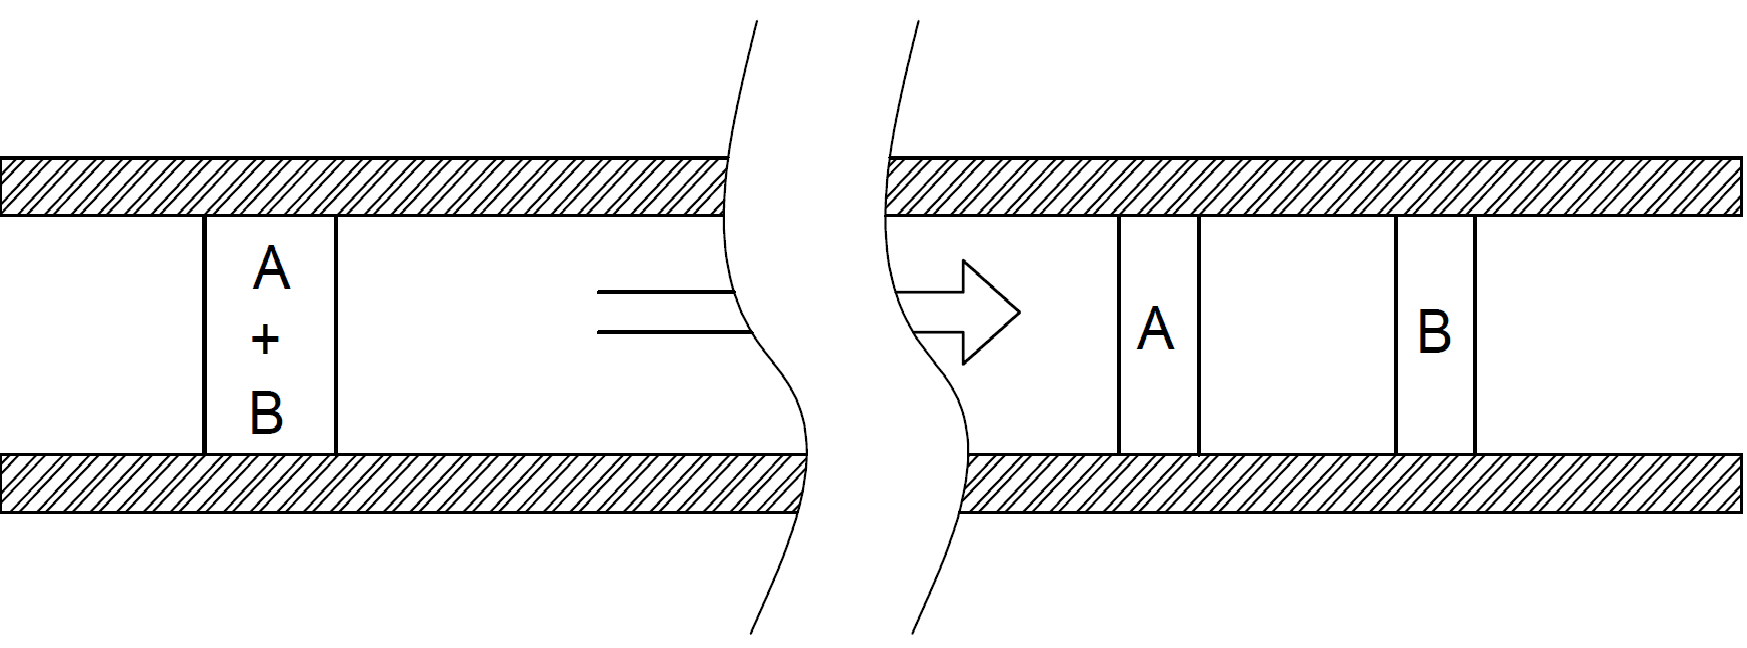
\includegraphics[width=0.5\textwidth]{column.png}
    %     \caption{Gas separation column}
    %     \label{fig:column}
    % \end{figure}

\subsection{Kubernetes}
\label{subsec:kube}

    Kubernetes stems from Google and has grown on the experience and challenges Google faced while building and maintaining their services, after two other closed sourced were build and used: Borg and Omega \cite{b9}. Kubernetes is open source and is not anymore managed by Google but by a foundation they have spinned up to oversee Kubernetes (and now they have hundreds of open source solutions in their landscape), called Cloud Native Computing Foundation or CNCF \cite{b11}.

    

\subsection{Service meshes}

\section{Implementation}

\begin{thebibliography}{00}

    \bibitem{b1} Hall, Richard S., Dennis Heimbigner, and Alexander L. Wolf. "A cooperative approach to support software deployment using the software dock." Proceedings of the 21st international conference on Software engineering. 1999.

    \bibitem{b2} Xuemei Zhang, Hoang Pham. "Software field failure rate prediction before software deployment, Journal of Systems and Software", Volume 79, Issue 3, 2006, Pages 291-300, ISSN 0164-1212.

    \bibitem{b3} A. Dearle. "Software Deployment, Past, Present and Future," Future of Software Engineering (FOSE '07), Minneapolis, MN, 2007, pp. 269-284. doi: 10.1109/FOSE.2007.20.

    \bibitem{b4} M. Conway, \href{https://en.wikipedia.org/wiki/Conway%27s_law}{Wikpedia, Conway's law page}

    \bibitem{b5} Thones, Johannes. "Microservices." IEEE software 32.1 (2015): 116-116.

    \bibitem{b6} Villamizar, Mario, et al. "Evaluating the monolithic and the microservice architecture pattern to deploy web applications in the cloud." 2015 10th Computing Colombian Conference (10CCC). IEEE, 2015.

    \bibitem{b7} Sheikh, Hammad, Ángel Gómez, and Scott Atran. "Empirical evidence for the devoted actor model." Current Anthropology 57.S13 (2016): S204-S209.

    \bibitem{b8} Docker. \href{https://www.docker.com}{Docker website}

    \bibitem{b9} Kubernetes. \href{https://kubernetes.io}{Kubernetes website}

    \bibitem{b10} Burns, Brendan, et al. "Borg, omega, and kubernetes." Queue 14.1 (2016): 70-93.

    \bibitem{b11} CNCF. \href{https://www.cncf.io}{CNCF website}
\end{thebibliography}
\vspace{12pt}

\end{document}
